% Options for packages loaded elsewhere
\PassOptionsToPackage{unicode}{hyperref}
\PassOptionsToPackage{hyphens}{url}
%
\documentclass[
]{article}
\usepackage{amsmath,amssymb}
\usepackage{iftex}
\ifPDFTeX
  \usepackage[T1]{fontenc}
  \usepackage[utf8]{inputenc}
  \usepackage{textcomp} % provide euro and other symbols
\else % if luatex or xetex
  \usepackage{unicode-math} % this also loads fontspec
  \defaultfontfeatures{Scale=MatchLowercase}
  \defaultfontfeatures[\rmfamily]{Ligatures=TeX,Scale=1}
\fi
\usepackage{lmodern}
\ifPDFTeX\else
  % xetex/luatex font selection
\fi
% Use upquote if available, for straight quotes in verbatim environments
\IfFileExists{upquote.sty}{\usepackage{upquote}}{}
\IfFileExists{microtype.sty}{% use microtype if available
  \usepackage[]{microtype}
  \UseMicrotypeSet[protrusion]{basicmath} % disable protrusion for tt fonts
}{}
\makeatletter
\@ifundefined{KOMAClassName}{% if non-KOMA class
  \IfFileExists{parskip.sty}{%
    \usepackage{parskip}
  }{% else
    \setlength{\parindent}{0pt}
    \setlength{\parskip}{6pt plus 2pt minus 1pt}}
}{% if KOMA class
  \KOMAoptions{parskip=half}}
\makeatother
\usepackage{xcolor}
\usepackage[top=20mm,bottom=20mm,left=15mm,right=15mm]{geometry}
\usepackage{graphicx}
\makeatletter
\def\maxwidth{\ifdim\Gin@nat@width>\linewidth\linewidth\else\Gin@nat@width\fi}
\def\maxheight{\ifdim\Gin@nat@height>\textheight\textheight\else\Gin@nat@height\fi}
\makeatother
% Scale images if necessary, so that they will not overflow the page
% margins by default, and it is still possible to overwrite the defaults
% using explicit options in \includegraphics[width, height, ...]{}
\setkeys{Gin}{width=\maxwidth,height=\maxheight,keepaspectratio}
% Set default figure placement to htbp
\makeatletter
\def\fps@figure{htbp}
\makeatother
\setlength{\emergencystretch}{3em} % prevent overfull lines
\providecommand{\tightlist}{%
  \setlength{\itemsep}{0pt}\setlength{\parskip}{0pt}}
\setcounter{secnumdepth}{-\maxdimen} % remove section numbering
\newlength{\cslhangindent}
\setlength{\cslhangindent}{1.5em}
\newlength{\csllabelwidth}
\setlength{\csllabelwidth}{3em}
\newlength{\cslentryspacingunit} % times entry-spacing
\setlength{\cslentryspacingunit}{\parskip}
\newenvironment{CSLReferences}[2] % #1 hanging-ident, #2 entry spacing
 {% don't indent paragraphs
  \setlength{\parindent}{0pt}
  % turn on hanging indent if param 1 is 1
  \ifodd #1
  \let\oldpar\par
  \def\par{\hangindent=\cslhangindent\oldpar}
  \fi
  % set entry spacing
  \setlength{\parskip}{#2\cslentryspacingunit}
 }%
 {}
\usepackage{calc}
\newcommand{\CSLBlock}[1]{#1\hfill\break}
\newcommand{\CSLLeftMargin}[1]{\parbox[t]{\csllabelwidth}{#1}}
\newcommand{\CSLRightInline}[1]{\parbox[t]{\linewidth - \csllabelwidth}{#1}\break}
\newcommand{\CSLIndent}[1]{\hspace{\cslhangindent}#1}
\usepackage{acl}
\usepackage{natbib}
\usepackage[inline]{enumitem}
\usepackage[justification=centering]{caption}
\bibliographystyle{acl_natbib.bst}
\setcounter{secnumdepth}{5}
\ifLuaTeX
  \usepackage{selnolig}  % disable illegal ligatures
\fi
\IfFileExists{bookmark.sty}{\usepackage{bookmark}}{\usepackage{hyperref}}
\IfFileExists{xurl.sty}{\usepackage{xurl}}{} % add URL line breaks if available
\urlstyle{same}
\hypersetup{
  pdfauthor={Ahmed Soliman; Marc Wenzlawski; Vladislav Yotkov},
  hidelinks,
  pdfcreator={LaTeX via pandoc}}

\title{Lay It On Me:

Generating Easy-to-Read Summaries for Non-Experts}
\author{Ahmed Soliman \and Marc Wenzlawski \and Vladislav Yotkov}
\date{}

\begin{document}
\maketitle
\begin{abstract}
In this project, we present an extractive-abstractive lay summarisation
pipeline for biomedical papers to generate accessible summaries for
non-experts. To achieve this, we construct a sentence-level dataset
optimized for maximizing ROUGE scores, utilizing lay summaries and
complete articles. We employ a BERT-based classifier to identify each
article's most critical sentences. The extracted summaries are then
input into two abstractive models, Clinical-Longformer and GPT-2, which
paraphrase the summaries to enhance readability. We evaluate the
performance of our models using the ROUGE metric and readability metrics
such as Flesch-Kincaid Grade Level (FKGL), Gunning Fog Score, and
Automated Readability Index (ARI). We find that a ROUGE-maximizing
extractive summarisation approach is practical for generating extractive
summaries, with the Clinical-Longformer model achieving the best results
for combined ROUGE and readability scores. Our approach demonstrates the
potential for generating lay-friendly summaries of biomedical papers,
bridging the gap between expert knowledge and public understanding.
\end{abstract}

\hypertarget{sec:introduction}{%
\section{Introduction}\label{sec:introduction}}

Comprehending biomedical scientific publications can be difficult for
non-experts, potentially leading to misinformed health decisions (Islam
et al. 2020). Lay summaries, simplified explanations of complex
scientific content, could be a solution, but they are not always
available. Despite past challenges in applying Automatic Text
Summarisation (ATS) to biomedicine due to insufficient data
(Chandrasekaran et al. 2020), two new datasets, PLOS and eLife, offer an
opportunity to bridge this gap (Goldsack et al. 2022). This study
investigates ATS techniques for generating biomedical lay summaries
using these datasets.

\hypertarget{sec:methods}{%
\section{Methods and Datasets}\label{sec:methods}}

In this section outline the various ATS methodologies employed in this
study and describe the PLOS and eLife datasets used for training and
evaluation purposes.

\hypertarget{sec:dataset}{%
\subsection{Dataset}\label{sec:dataset}}

The data we used is sourced from biomedical research articles in English
published in the Public Library of Science (PLOS) and eLife (Goldsack et
al. 2022). The datasets (Tables \ref{tab:dataset_stats_1} and
\ref{tab:dataset_stats_2}) contain technical abstracts and lay summaries
written by experts, which are part of BioLaySumm2023 shared task
(Goldsack et al. 2023).

\begin{table}[htbp]
    \centering
    \begin{tabular}{|c|c|c|}
        \hline
        \textbf{Dataset} & \textbf{Training} & \textbf{Validation} \\
        \hline
            PLOS & $24,773$ & $1,376$ \\
        \hline
            eLife & $4,346$ & $241$ \\
        \hline
    \end{tabular}
    \caption{PLOS and eLife: number of articles}\label{tab:dataset_stats_1}
\end{table}

\begin{table}[htbp]
    \centering
    \begin{tabular}{|c|c|c|}
        \hline
        \textbf{Dataset} & \textbf{Avg. Sentences} & \textbf{Avg. Tokens} \\
        \hline
            PLOS & $300$ & $9,000$ \\
        \hline
            eLife & $600$ & $14,000$ \\
        \hline
    \end{tabular}
    \caption{PLOS and eLife: Dataset statistics}\label{tab:dataset_stats_2}
\end{table}

\hypertarget{sec:extractor-network}{%
\subsection{Extractor Network}\label{sec:extractor-network}}

Due to the extreme length of medical articles (e.g., eLife has an
average of \(600\) sentences per article), it is not feasible to pass
them directly as input to the abstractive models due to their limited
maximum input size:

\begin{enumerate}
\def\labelenumi{\roman{enumi}.}
\tightlist
\item
  \textbf{GPT-2} (Radford et al. 2019a): \(1,024\) tokens, and
\item
  \textbf{Clinical-Longformer} (Li et al. 2023): \(4,096\) tokens
\end{enumerate}

To overcome this limitation, we use the BioClinicalBERT (Alsentzer et
al. 2019) model, pre-trained on the MIMIC-III dataset (Johnson et al.
2016), to extract the most important sentences from the articles. For
that purpose, we cast the extraction summarisation problem as supervised
binary classification where the input is a sentence \(s\) and the output
is a binary label indicating whether the sentence should be included in
the summary \(c\) or not (i.e., \(1\) and \(0\), respectively). Due to
the nature of the provided gold summaries (i.e., abstractive and lay),
we generate our own sentence-level dataset by applying the
ROUGE-maximisation technique (Zmandar et al. 2021; Nallapati, Zhai, and
Zhou 2017) on the gold summaries and the whole articles. More formally,
for each gold summary sentence \(s_{i}^{k}\), we find the sentence
\(s_{j}^{k}\) in article \(a_{k}\) that maximises the ROUGE-2 score
between them. We then label \(s_{j}^{k}\) as \(1\) and the rest of the
sentences in \(a_{k}\) as \(0\). Because the number of sentences in the
articles is much larger than the number of sentences in the gold
summaries:

\begin{enumerate}
\def\labelenumi{\roman{enumi}.}
\tightlist
\item
  We base our extractive binary dataset on both eLife and PLOS data to
  maximise the number of training samples;
\item
  We further resolve the class imbalance problem by random
  under-sampling the majority class (i.e., \(0\)) to match the number of
  samples in the minority class (i.e., \(1\));
\end{enumerate}

Our final extractive dataset consists of \(944,234\) sentences with a
completely balanced class distribution. Data is further split into
\(80\%\)-training, \(10\%\)-validation and \(10\%\)-testing datasets in
a random stratified manner. We then fine-tune the extractive model with
a batch size of \(32\) and a learning rate of \(2 \times 10^{-5}\)
following the guidance from BERT's authors (Devlin et al. 2019) and find
that the model starts to over-fit beyond \(2\) epochs (see Figures
\ref{fig:extractor-eval-f1} and \ref{fig:extractor-eval-loss}). We also
report high F1 scores of \(0.767\) and \(0.765\) on the validation and
test sets, respectively.

\begin{figure}
    \centering
    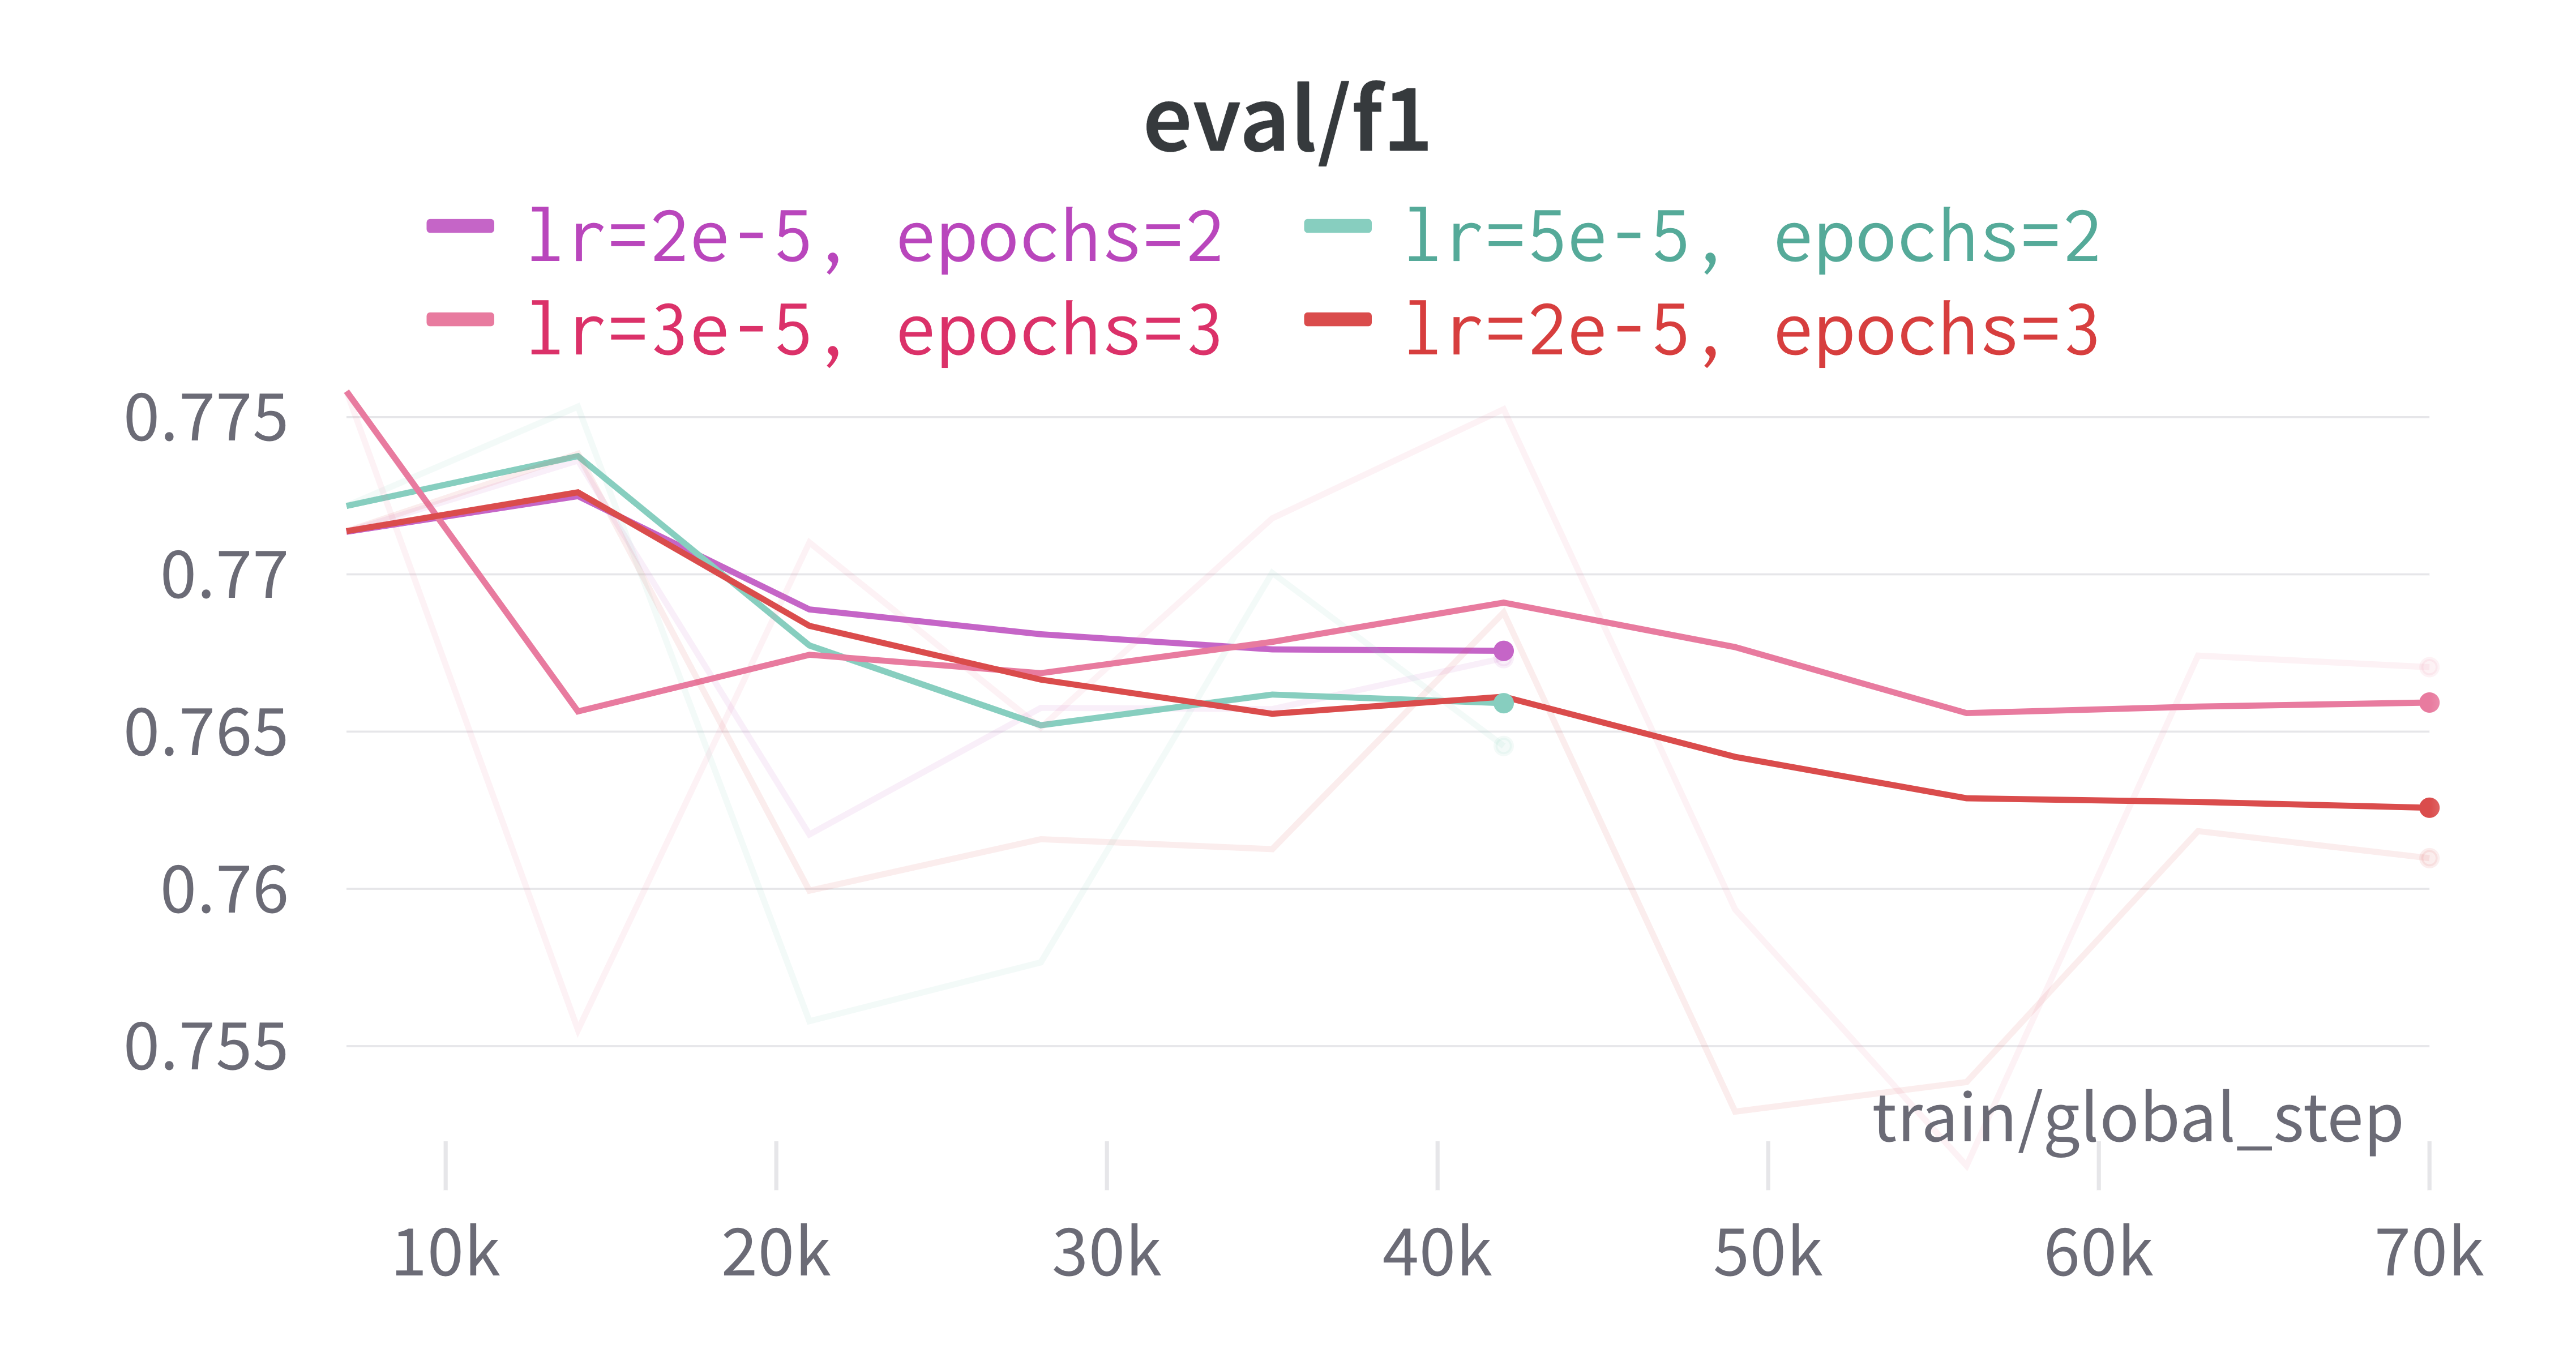
\includegraphics[width=0.5\textwidth]{charts/extractor-eval-f1.png}
    \caption{BioClinicalBERT: Evaluation F1}\label{fig:extractor-eval-f1}
    \vspace{0.25cm}
    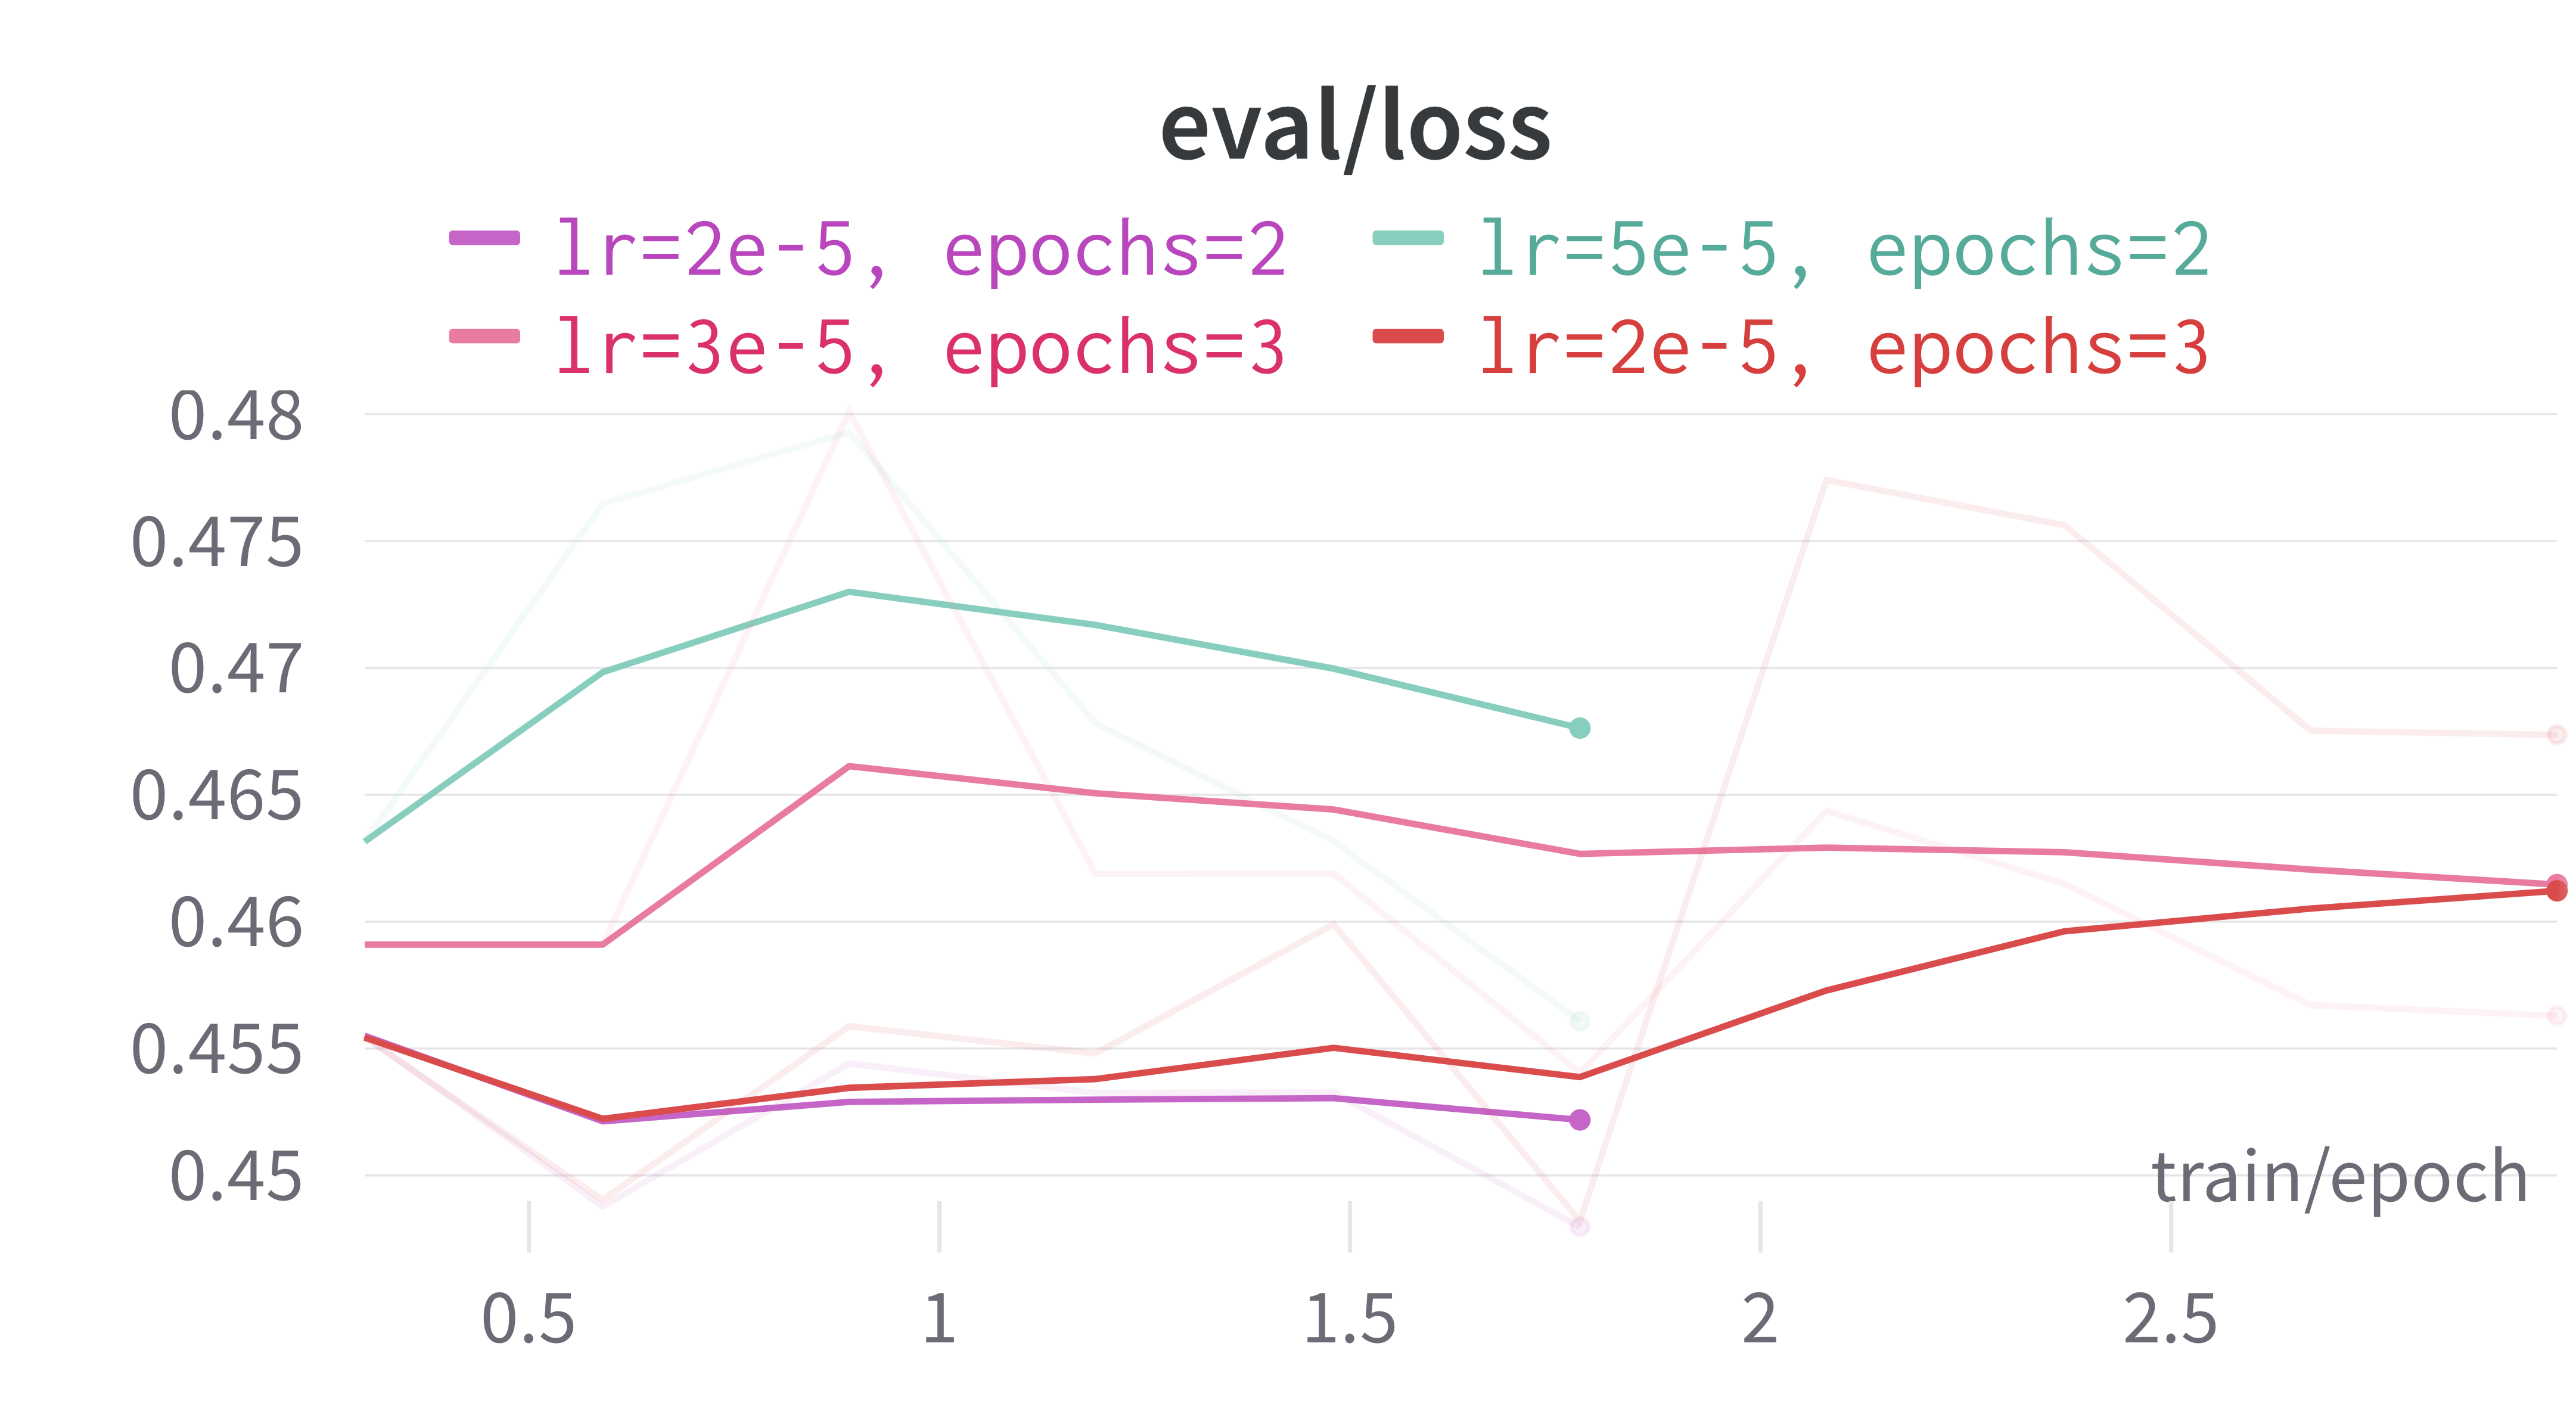
\includegraphics[width=0.5\textwidth]{charts/extractor-eval-loss.png}
    \caption{BioClinicalBERT: Evaluation Loss}\label{fig:extractor-eval-loss}
\end{figure}

We then use the BioClinicalBERT model to predict the probability of each
sentence in the article being \emph{summarising}. The top \(10\) with
the highest probability are selected and concatenated to produce the
final extractive summary. We arrive at this number after analysing the
token distribution and finding that \(10\) sentences is a reasonable
number to fit within the maximum input size of the GPT-2 abstractive
model (i.e., \(1,024\) tokens split between the ten sentences and their
lay paraphrases). We also experiment with a top-\(15\) strategy only for
the Clinical Longformer to fully make use of the sparse attention
mechanism (see Section \ref{sec:evaluation-quantitative}). While we are
aware that this can cause the \emph{dangling anaphora phenomenon} (Lin
2009), we use the extracted text only as an intermediate step fed into
the abstractive models, paraphrasing it into lay language.

\hypertarget{sec:abstractive-network}{%
\subsection{Abstractive Network}\label{sec:abstractive-network}}

Once the extractive summary is generated, we train the abstractive
models on the lay summaries and the extractive summaries. For this, we
compare two models: GPT-2 (Radford et al. 2019a) and Clinical-Longformer
(Li et al. 2022). We fine-tune both models separately on eLife and PLOS.
This is done due to the difference in structure and the average number
of tokens in the lay summaries between the two datasets (i.e., \(450\)
and \(800\) for PLOS and eLife, respectively). Hyperparameters are set
based on widely used values in the literature (Li et al. 2022; Radford
et al. 2019a; Devlin et al. 2019).

\hypertarget{sec:clinical-longformer-abstractor}{%
\subsubsection{Clinical Longformer
Abstractor}\label{sec:clinical-longformer-abstractor}}

The Clinical Longformer (Li et al. 2023) is a transformer-based model
that is pre-trained on the MIMIC-III dataset (Johnson et al. 2016) and
can process up to \(4,096\) tokens in a single input sequence. This is
achieved by implementing a sparse attention mechanism that allows more
computationally efficient processing of long-range dependencies. We
fine-tune the Clinical Longformer as a sequence-to-sequence task on
pairs of (a) gold lay summaries and (b) ROUGE-maximising training data
described in Section \ref{sec:extractor-network}.

\begin{figure}
    \centering
    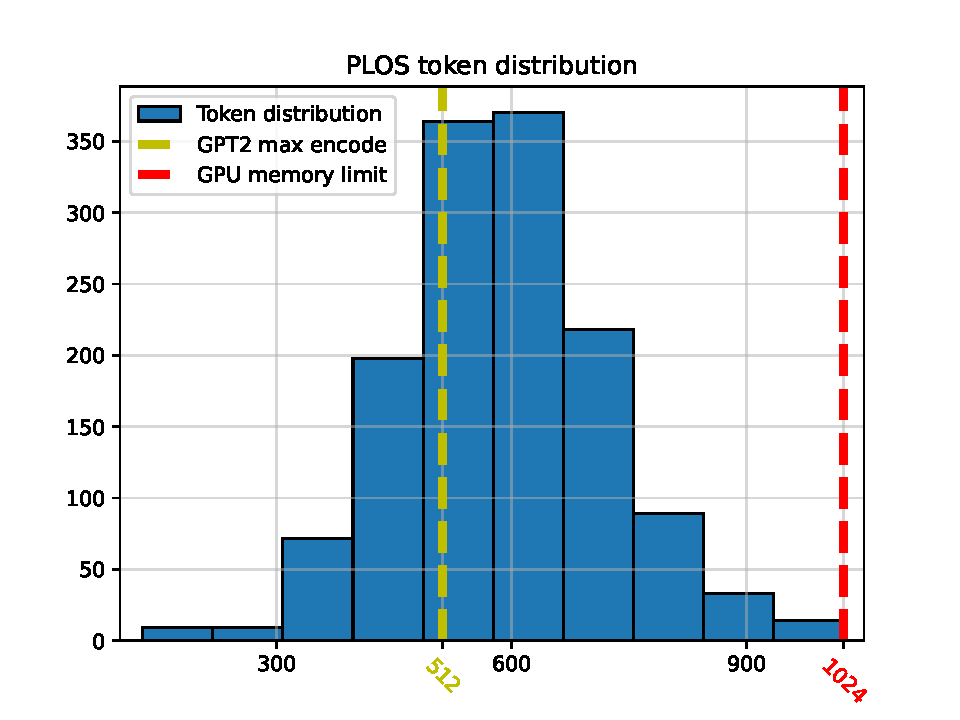
\includegraphics[width=0.5\textwidth]{charts/token_distribution}
    \caption{Token Distribution of Extracted Summaries}\label{fig:abstractor-eval-rouge}
\end{figure}

For the Longformer model, we experimented with window, batch, and input
size to ensure that we would not run out of memory during training, as
this is a common issue with such models (Orzhenovskii 2021). We found
that a window size of \(32\), batch size of \(1\), and input size of
\(1,024\) worked best for our dataset, resulting in an evaluation loss
of \(3.4\) (Figure \ref{fig:abstractor-eval-loss}).

\begin{figure}
    \centering
    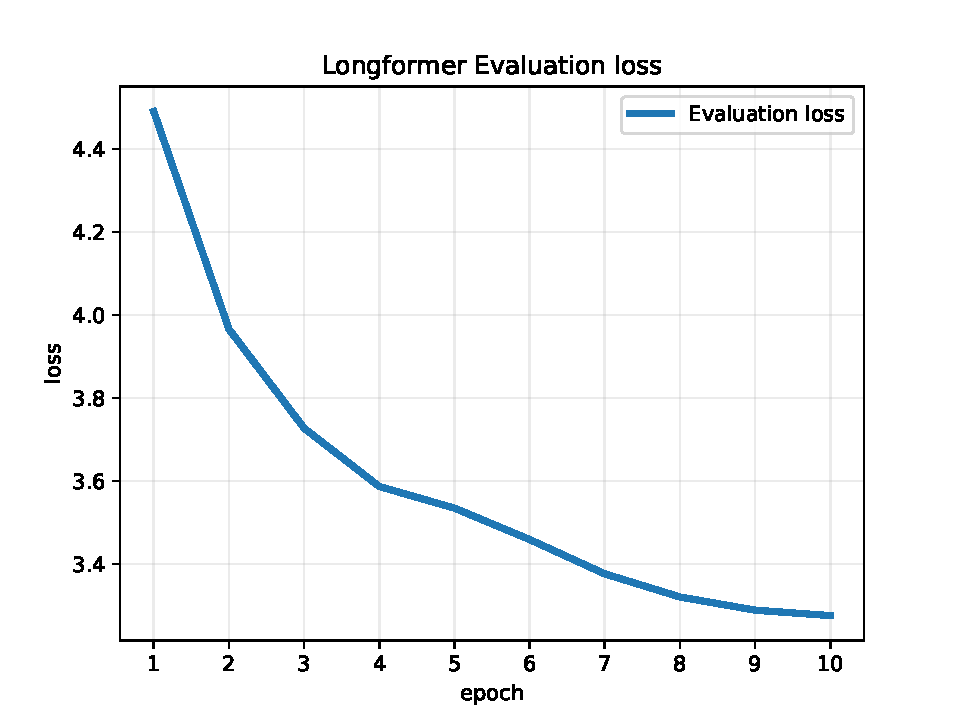
\includegraphics[width=0.49\textwidth]{charts/lf_eval_loss}
    \caption{Longformer evaluation loss}\label{fig:abstractor-eval-loss}
\end{figure}

\hypertarget{sec:gpt2-abstractor}{%
\subsubsection{GPT-2 Abstractor}\label{sec:gpt2-abstractor}}

The GPT-2 is an autoregressive language model that was trained using a
casual language modelling objective (Radford et al. 2019b). Given its
extensive exposure to diverse text sources and natural language
patterns, we hypothesize that GPT-2 would be particularly adept at
generating lay summaries, making it a promising candidate for the
abstractive summarisation task. To fine-tune GPT-2 for this purpose, we
utilize a ``TL;DR'' prompt, instructing the model to generate concise
and informative summaries.

Similar to the Longformer, we train GPT-2 on both eLife and PLOS
datasets, adopting most hyperparameters from the existing literature to
ensure optimal performance (Bajaj et al. 2021). Since GPT-2 can
accommodate 1024 tokens, we experimented with various splits between the
number of tokens allocated for the extracted summary and the lay
summary. Through experimentation, we determined that allocating \(507\)
tokens for the article and \(512\) tokens for the summary, with \(5\)
reserved for the ``TL;DR'' prompt, yielded the best results regarding
summary quality and model performance. Figure \ref{fig:gpt-eval}
illustrates the evaluation loss decrease during the fine-tuning process.

\begin{figure}
    \centering
    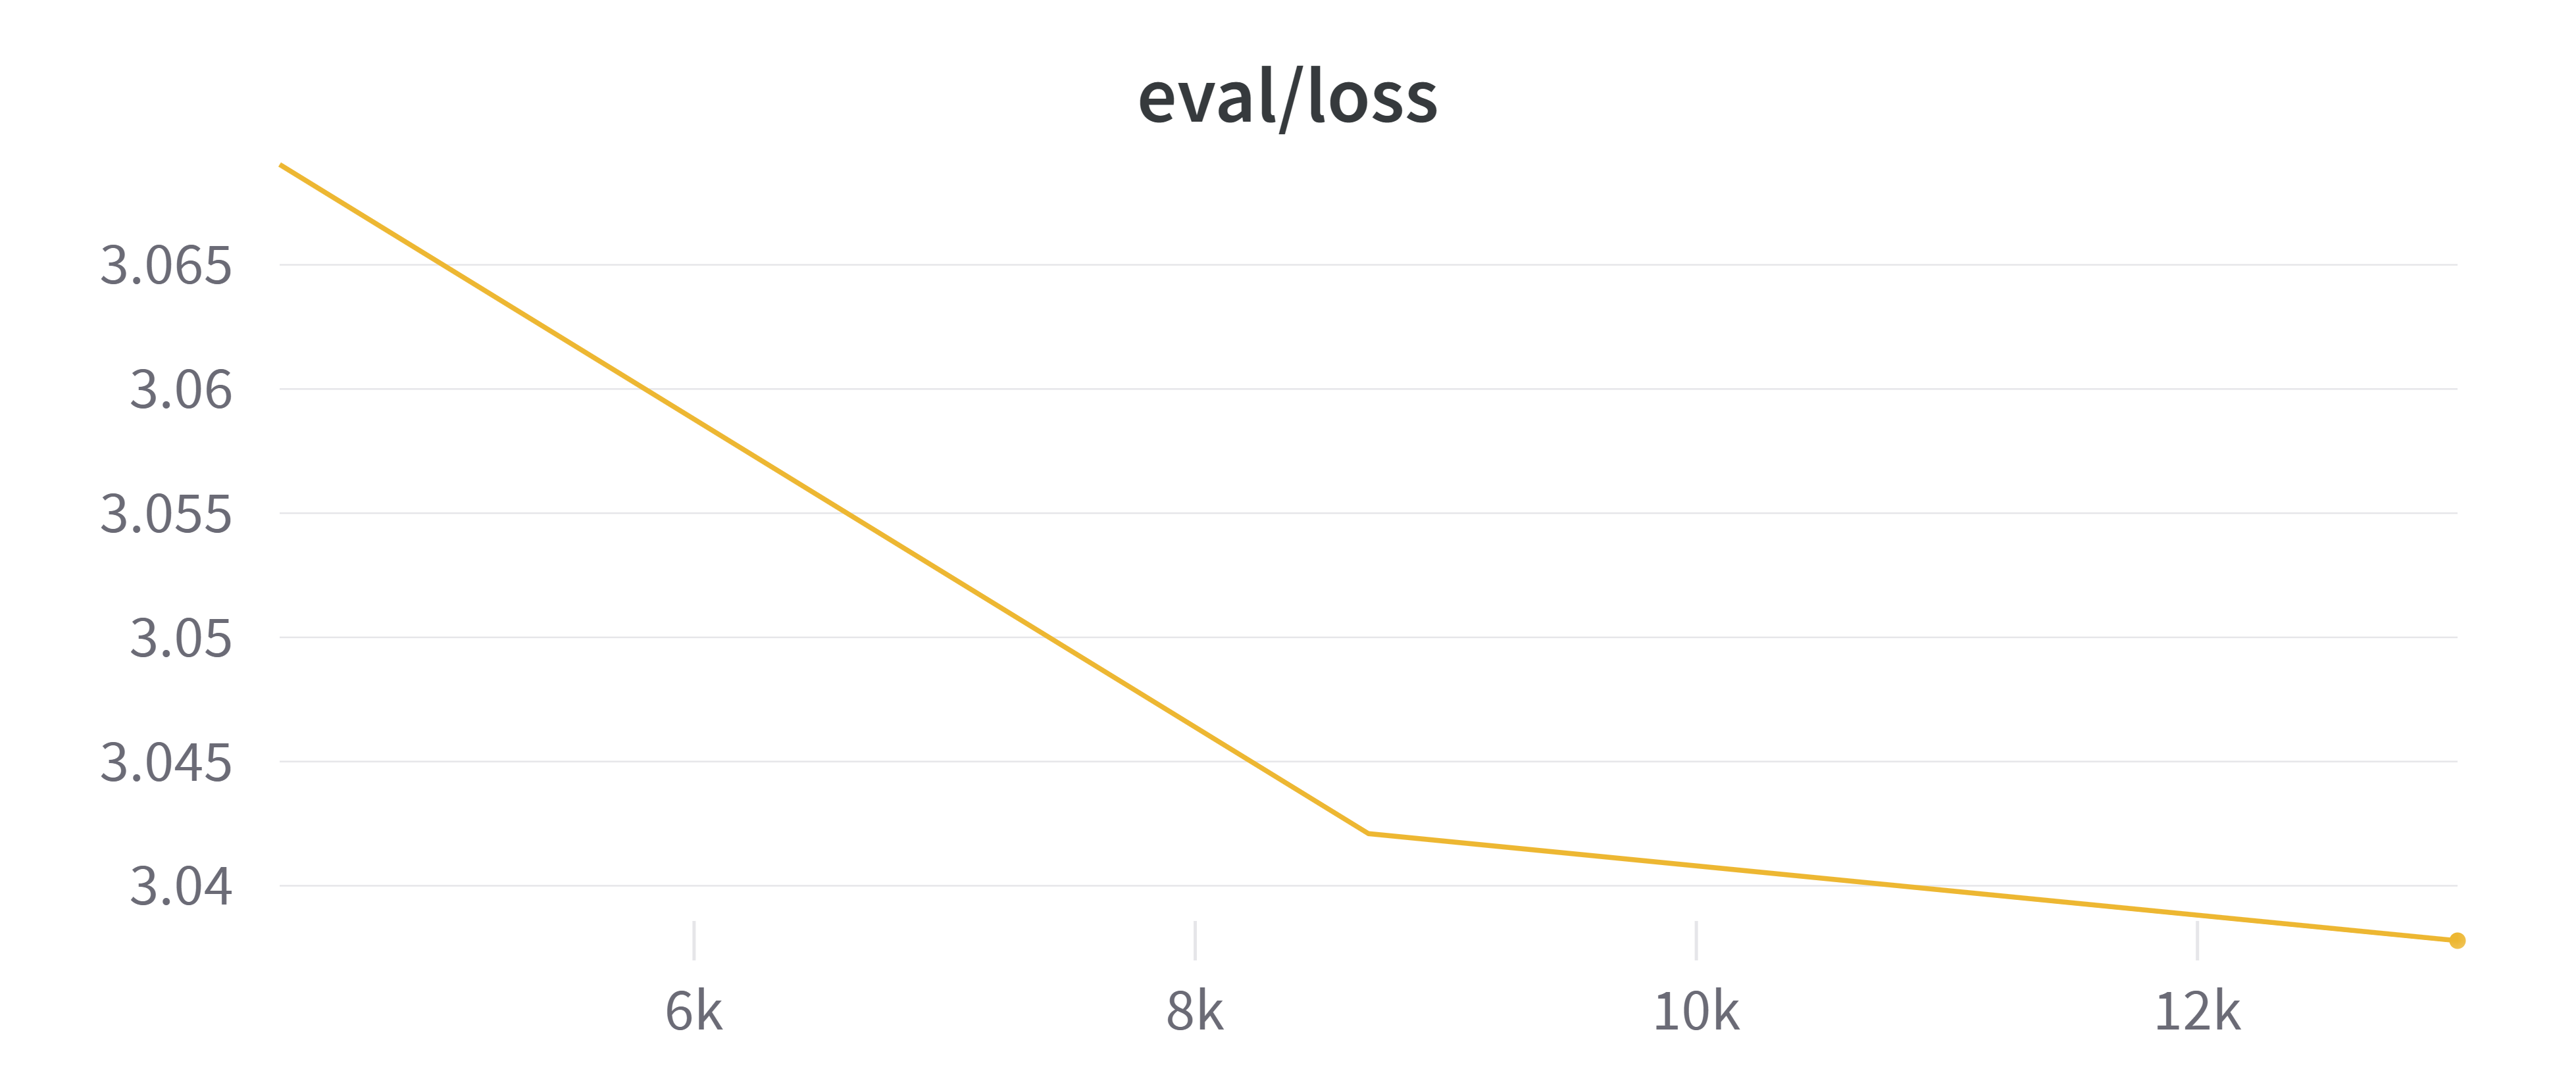
\includegraphics[width=0.49\textwidth]{charts/gpt_eval_loss}
    \caption{GPT 2 Evaluation Loss}\label{fig:gpt-eval}
\end{figure}

In the evaluation phase, we compared the performance of the GPT-2
Abstractor against the Clinical Longformer Abstractor, as well as other
summarisation models. The results indicate that both models have their
strengths and weaknesses, which we will discuss in further detail in the
following sections.

\hypertarget{sec:evaluation}{%
\section{Evaluation}\label{sec:evaluation}}

In this section, we evaluate the performance of the summarisation models
described in Section \ref{sec:methods}.

\hypertarget{sec:evaluation-quantitative}{%
\subsection{Quantitative Evaluation}\label{sec:evaluation-quantitative}}

We compare our models by calculating the average F1 ROUGE scores on the
PLOS evaluation dataset. From Table \ref{tab:dataset_stats}, we can see
that our Extractive Network performs as well as the standard ATS
baseline - LexRank (Erkan and Radev 2004) in terms of the lexical
overlap with the gold lay summary. On the other hand, we observe that
the metrics decrease for the generative models due to their abstractive
nature, which demonstrates how problematic and inconvenient for lay
summarisation ROUGE is. Nevertheless, the Clinical Longformer
outperforms the GPT-2, perhaps because the latter is pre-trained on
out-of-domain data. Furthermore, we also note insignificant differences
in ROUGE between the top-10 and top-15 strategies of Sentence Extraction
(see Section \ref{sec:extractor-network}) for the Clinical Longformer.

\begin{table}[htbp]
    \centering
    \begin{tabular}{|c|c|c|c|}
        \hline
        \textbf{Model} & \textbf{Rouge1} & \textbf{Rouge2} & \textbf{RougeL} \\
        \hline
            Lexrank & $\textbf{0.34}$ & $0.09$ & $\textbf{0.16}$ \\
        \hline
            Extractive & $0.33$ & $\textbf{0.10}$ & $\textbf{0.16}$ \\
        \hline
            GPT2 & $0.18$ & $0.02$ & $0.09$ \\
        \hline
            Longformer (top-15) & $0.28$ & $0.07$ & $0.15$ \\
        \hline
            Longformer (top-10) & $0.29$ & $0.06$ & $0.14$ \\
        \hline
    \end{tabular}
    \caption{ROUGE F1 Scores.}\label{tab:dataset_stats}
\end{table}

Regarding the readability of the generated summaries, it is clear and
expected that our Extracted summary results in a low FKGL (Kincaid et
al. 1975) and a high ARI (Senter and Smith 1967) - meaning that it
contains a lot of scientific jargon and is hard to read. On the other
hand, the GPT-2 and Longformer successfully manage to transform the
extracted output into a more lay language with significant improvements
in readability. Surprisingly, the top-10 strategy of the Clinical
Longformer results in better lay summarisation than the top-15 one. We
argue that this is caused by the smaller number of highly-technical and
unrelated extracted sentences (top-10) that the model has to deal with.
We remind the reader that in the provided dataset, 15 sentences amounts
to the maximum number of tokens that can be fed to the Longformer model
- \(1,024\) (due to computational limitations).

\begin{table}[htbp]
    \centering
    \begin{tabular}{|c|c|c|c|}
        \hline
        \textbf{Model} & \textbf{FKGL} & \textbf{ARI} & \textbf{Gunning} \\
        \hline
            Lay & 20.01 & 16.50 & 19.11 \\
        \hline
            Lex (Baseline) & \textbf{33.58} & \textbf{15.41} & 18.50 \\
        \hline
            Extractive & 10.60 & 25.01 & 26.22 \\
        \hline
            GPT2 & 30.68 & 21.36 & 23.26 \\
        \hline
            Longformer (top-15) & 23.84 & 19.62 & 20.62 \\
        \hline
            Longformer (top-10) & $27.33$ & $16.89$ & $\textbf{18.44}$ \\
        \hline
    \end{tabular}
    \caption{Readability metrics. \\ FKGL - higher is better, ARI and Gunning - lower is better}\label{tab:dataset_stats}
\end{table}

\hypertarget{sec:evaluation-qualitative}{%
\subsection{Qualitative Evaluation}\label{sec:evaluation-qualitative}}

Our qualitative evaluation revealed that extractive summarisation often
encounters a dangling anaphora problem, which can lead to confusion.
However, we observed that the Longformer could generate coherent
summaries that matched the original content. Despite this, as the
Longformer-produced summaries progressed, they tended to drift away from
the lay summary's intent and exhibited repetitive information leading to
lengthy summaries

Conversely, the GPT model exhibited significant variability in its
results. It frequently misinterpreted clinical terms, hallucinated
summaries with incorrect or fabricated information, and was fixated on
specific characters, tables, and mathematical symbols rather than the
core content. While the GPT model achieved higher readability metrics by
employing simpler terms, the summaries were often nonsensical and
difficult to understand.

\hypertarget{sec:discussion-conclusion}{%
\section{Discussion}\label{sec:discussion-conclusion}}

In this section, we discuss the performance of the proposed ATS
approaches, their implications, and potential future research directions
in the biomedical domain.

\hypertarget{sec:limitations}{%
\subsection{Limitations}\label{sec:limitations}}

We identify the following limitations of our work:

\textbf{Readability Evaluation}: Although, we are evaluating our models
with the traditional metrics: FKGL (Kincaid et al. 1975), ARI (Senter
and Smith 1967), and Gunning (Gunning 1952), they are insufficient for
the estimation of text readability in scientific writing. Instead, what
some researchers propose is to leverage masked language models (Martinc,
Pollak, and Robnik-Šikonja 2021) like the noun-phrase BERT-based metric
(Luo, Xie, and Ananiadou 2022) that computes the probability of
technical jargon. We appreciate that this method would have provided a
more thorough evaluation of our models, and we leave it as future work.

\textbf{Limited input size}: Due to the limited available computational
resources (i.e., Tesla V100-SXM2-16GB) we had to restrict the input size
of the Longformer to \(1,024\) tokens (i.e., \(4\) times less than the
maximum size). Therefore, we could not make use of the full model
capabilities in attending to long-range dependencies. This limitation
propagates back to our extractor network, which produces only enough
sentences to fit in the abstractor network. Thus, if we could increase
the Longformer's input size, we could do the same for the Extractor
model.

\hypertarget{sec:future-work}{%
\subsection{Future Work}\label{sec:future-work}}

In light of the limitations discussed, we propose multiple venues for
future work:

\textbf{T5 Experimentation} (Lehman and Johnson 2023): We aim to develop
and assess the Clinical T5 model as a specialized counterpart to the
Clinical Longformer. The T5, a transformer-based model, boasts unique
features like a denoising autoencoder in its pretraining objective,
which is adept at reconstructing corrupted input text. This makes it
suitable for our extractive approach, utilising sentences from disparate
article sections.

\textbf{Clinical Longformer Enhancement} (Li et al. 2022): Our goal is
to augment the Clinical Longformer's maximum token capacity by employing
advanced hardware resources. This would facilitate experimentation with
larger input dimensions and model training, potentially leading to
superior summarisation performance and more precise lay summaries.

\textbf{Feedback Integration}: We suggest incorporating readability and
factual correctness rewards into our summarisation pipeline using
reinforcement learning methods (Scialom et al. 2019). This can be
achieved by the combination of the RNPTC metric (Luo, Xie, and Ananiadou
2022) and the factual accuracy (Zhang et al. 2020) into a single reward
function, optimised via the Reinforce algorithm (Williams 1992). This
approach aspires to promote the generation of summaries that are not
only more comprehensible for non-experts but also more correct with
respect to the input article.

\hypertarget{sec:conclusion}{%
\section{Conclusion}\label{sec:conclusion}}

Our project presents an effective two-step approach for generating lay
summaries of biomedical research articles. We incorporate an extraction
step using the BioClinicalBERT model and an abstractive step using
either GPT-2 or Clinical Longformer models.

Results indicate that the classifier trained on the ROUGE-maximising
dataset performs well in extracting relevant sentences. At the same
time, the Clinical Longformer Abstractor can generate coherent lay
summaries, achieving a good balance between ROUGE and readability
scores. This suggests that an extractive abstractive approach to lay
summarisation effectively generates lay summaries while reducing
computational costs.

\hypertarget{bibliography}{%
\section*{Bibliography}\label{bibliography}}
\addcontentsline{toc}{section}{Bibliography}

\hypertarget{refs}{}
\begin{CSLReferences}{1}{0}
\leavevmode\vadjust pre{\hypertarget{ref-alsentzer-etal-2019-publicly}{}}%
Alsentzer, Emily, John Murphy, William Boag, Wei-Hung Weng, Di Jin,
Tristan Naumann, and Matthew McDermott. 2019. {``Publicly Available
Clinical {BERT} Embeddings.''} In \emph{Proceedings of the 2nd Clinical
Natural Language Processing Workshop}, 72--78. Minneapolis, Minnesota,
USA: Association for Computational Linguistics.
\url{https://doi.org/10.18653/v1/W19-1909}.

\leavevmode\vadjust pre{\hypertarget{ref-bajaj-etal-2021-long}{}}%
Bajaj, Ahsaas, Pavitra Dangati, Kalpesh Krishna, Pradhiksha Ashok Kumar,
Rheeya Uppaal, Bradford Windsor, Eliot Brenner, Dominic Dotterrer,
Rajarshi Das, and Andrew McCallum. 2021. {``Long Document Summarization
in a Low Resource Setting Using Pretrained Language Models.''} In
\emph{Proceedings of the 59th Annual Meeting of the Association for
Computational Linguistics and the 11th International Joint Conference on
Natural Language Processing: Student Research Workshop}, 71--80. Online:
Association for Computational Linguistics.
\url{https://doi.org/10.18653/v1/2021.acl-srw.7}.

\leavevmode\vadjust pre{\hypertarget{ref-chandrasekaran}{}}%
Chandrasekaran, Muthu Kumar, Guy Feigenblat, Eduard Hovy, Abhilasha
Ravichander, Michal Shmueli-Scheuer, and Anita de Waard. 2020.
{``Overview and Insights from the Shared Tasks at Scholarly Document
Processing 2020: {CL}-{S}ci{S}umm, {L}ay{S}umm and {L}ong{S}umm.''} In
\emph{Proceedings of the First Workshop on Scholarly Document
Processing}, 214--24. Online: Association for Computational Linguistics.
\url{https://doi.org/10.18653/v1/2020.sdp-1.24}.

\leavevmode\vadjust pre{\hypertarget{ref-Devlin2019BERTPO}{}}%
Devlin, Jacob, Ming-Wei Chang, Kenton Lee, and Kristina Toutanova. 2019.
{``BERT: Pre-Training of Deep Bidirectional Transformers for Language
Understanding.''} \emph{ArXiv} abs/1810.04805.

\leavevmode\vadjust pre{\hypertarget{ref-erkan2004}{}}%
Erkan, Günes, and Dragomir R. Radev. 2004. {``LexRank: Graph-Based
Lexical Centrality as Salience in Text Summarization.''} \emph{J. Artif.
Int. Res.} 22 (1): 457--79.

\leavevmode\vadjust pre{\hypertarget{ref-biolaysumm-2023-overview}{}}%
Goldsack, Tomas, Zheheng Luo, Qianqian Xie, Carolina Scarton, Matthew
Shardlow, Sophia Ananiadou, and Chenghua Lin. 2023. {``Overview of the
BioLaySumm 2023 Shared Task on Lay Summarization of Biomedical Research
Articles.''} In \emph{Proceedings of the 22st Workshop on Biomedical
Language Processing}. Toronto, Canada: Association for Computational
Linguistics.

\leavevmode\vadjust pre{\hypertarget{ref-goldsack}{}}%
Goldsack, Tomas, Zhihao Zhang, Chenghua Lin, and Carolina Scarton. 2022.
{``Making Science Simple: Corpora for the Lay Summarisation of
Scientific Literature.''} In \emph{Proceedings of the 2022 Conference on
Empirical Methods in Natural Language Processing}, 10589--604. Abu
Dhabi, United Arab Emirates: Association for Computational Linguistics.
\url{https://aclanthology.org/2022.emnlp-main.724}.

\leavevmode\vadjust pre{\hypertarget{ref-gunning1952technique}{}}%
Gunning, Robert. 1952. \emph{The Technique of Clear Writing}. New York:
McGraw-Hill.

\leavevmode\vadjust pre{\hypertarget{ref-islam}{}}%
Islam, Md Saiful, Tonmoy Sarkar, Sazzad Hossain Khan, Abu-Hena Mostofa
Kamal, Sarkar Mohammad Murshid Hasan, Alamgir Kabir, Dalia Yeasmin, et
al. 2020. {``COVID-19--Related Infodemic and Its Impact on Public
Health: A Global Social Media Analysis.''} \emph{The American Journal of
Tropical Medicine and Hygiene} 103 (4).
https://doi.org/\url{https://doi.org/10.4269/ajtmh.20-0812}.

\leavevmode\vadjust pre{\hypertarget{ref-Johnson2016MIMICIII}{}}%
Johnson, A. E. W., T. J. Pollard, L. Shen, L. W. Lehman, M. Feng, M.
Ghassemi, B. Moody, P. Szolovits, L. A. Celi, and R. G. Mark. 2016.
{``MIMIC-III, a Freely Accessible Critical Care Database.''}
\emph{Scientific Data} 3: 160035.
\url{https://doi.org/10.1038/sdata.2016.35}.

\leavevmode\vadjust pre{\hypertarget{ref-Kincaid1975DerivationON}{}}%
Kincaid, J. Peter, Robert P. Fishburne, Richard L. Rogers, and Brad S.
Chissom. 1975. {``Derivation of New Readability Formulas (Automated
Readability Index, Fog Count and Flesch Reading Ease Formula) for Navy
Enlisted Personnel.''} In.

\leavevmode\vadjust pre{\hypertarget{ref-clinicalt5}{}}%
Lehman, Eric, and Alistair Johnson. 2023. {``Clinical-T5: Large Language
Models Built Using MIMIC Clinical Text V1.0.0.''} \emph{Physionet.org}.
\url{https://physionet.org/content/clinical-t5/1.0.0/}.

\leavevmode\vadjust pre{\hypertarget{ref-li2022clinicallongformer}{}}%
Li, Yikuan, Ramsey M. Wehbe, Faraz S. Ahmad, Hanyin Wang, and Yuan Luo.
2022. {``Clinical-Longformer and Clinical-BigBird: Transformers for Long
Clinical Sequences.''} \url{https://arxiv.org/abs/2201.11838}.

\leavevmode\vadjust pre{\hypertarget{ref-li2023comparative}{}}%
Li, Yikuan, Ramsey M Wehbe, Faraz S Ahmad, Hanyin Wang, and Yuan Luo.
2023. {``A Comparative Study of Pretrained Language Models for Long
Clinical Text.''} \emph{Journal of the American Medical Informatics
Association} 30 (2): 340--47.

\leavevmode\vadjust pre{\hypertarget{ref-lin2009summarization}{}}%
Lin, Jimmy. 2009. {``Summarization.''} In \emph{Encyclopedia of Database
Systems}, 2906--10. Heidelberg, Germany: Springer.

\leavevmode\vadjust pre{\hypertarget{ref-luo}{}}%
Luo, Zheheng, Qianqian Xie, and Sophia Ananiadou. 2022. {``Readability
Controllable Biomedical Document Summarization.''} In \emph{Findings of
the Association for Computational Linguistics: EMNLP 2022}, 4667--80.
Abu Dhabi, United Arab Emirates: Association for Computational
Linguistics. \url{https://aclanthology.org/2022.findings-emnlp.343}.

\leavevmode\vadjust pre{\hypertarget{ref-martinc_readability}{}}%
Martinc, Matej, Senja Pollak, and Marko Robnik-Šikonja. 2021.
{``{Supervised and Unsupervised Neural Approaches to Text
Readability}.''} \emph{Computational Linguistics} 47 (1): 141--79.
\url{https://doi.org/10.1162/coli_a_00398}.

\leavevmode\vadjust pre{\hypertarget{ref-nallapati2017summarunner}{}}%
Nallapati, Ramesh, Feifei Zhai, and Bowen Zhou. 2017. {``SummaRuNNer: A
Recurrent Neural Network Based Sequence Model for Extractive
Summarization of Documents.''} In \emph{Proceedings of the Thirty-First
AAAI Conference on Artificial Intelligence}, 3075--81. AAAI'17. San
Francisco, California, USA: AAAI Press.

\leavevmode\vadjust pre{\hypertarget{ref-orzhenovskii-2021-t5}{}}%
Orzhenovskii, Mikhail. 2021. {``T5-{LONG}-{EXTRACT} at {FNS}-2021 Shared
Task.''} In \emph{Proceedings of the 3rd Financial Narrative Processing
Workshop}, 67--69. Lancaster, United Kingdom: Association for
Computational Linguistics. \url{https://aclanthology.org/2021.fnp-1.12}.

\leavevmode\vadjust pre{\hypertarget{ref-radford2019language}{}}%
Radford, Alec, Jeff Wu, Rewon Child, David Luan, Dario Amodei, and Ilya
Sutskever. 2019a. {``Language Models Are Unsupervised Multitask
Learners.''}

\leavevmode\vadjust pre{\hypertarget{ref-radford_wu}{}}%
Radford, Alec, Jeffrey Wu, Rewon Child, David Luan, Dario Amodei, and
Ilya Sutskever. 2019b. \emph{Language Models Are Unsupervised Multitask
Learners}.
\url{https://cdn.openai.com/better-language-models/language_models_are_unsupervised_multitask_learners.pdf}.

\leavevmode\vadjust pre{\hypertarget{ref-scialom-etal-2019-answers}{}}%
Scialom, Thomas, Sylvain Lamprier, Benjamin Piwowarski, and Jacopo
Staiano. 2019. {``Answers Unite! Unsupervised Metrics for Reinforced
Summarization Models.''} In \emph{Proceedings of the 2019 Conference on
Empirical Methods in Natural Language Processing and the 9th
International Joint Conference on Natural Language Processing
(EMNLP-IJCNLP)}, 3246--56. Hong Kong, China: Association for
Computational Linguistics. \url{https://doi.org/10.18653/v1/D19-1320}.

\leavevmode\vadjust pre{\hypertarget{ref-senter1967automated}{}}%
Senter, R J, and E A Smith. 1967.
{``\href{https://www.ncbi.nlm.nih.gov/pubmed/5302480}{Automated
Readability Index}.''} AMRL-TR-6620. Wright-Patterson Air Force Base:
Aerospace Medical Research Laboratories (U.S.).

\leavevmode\vadjust pre{\hypertarget{ref-williams1992simple}{}}%
Williams, Ronald J. 1992. {``Simple Statistical Gradient-Following
Algorithms for Connectionist Reinforcement Learning.''} \emph{Mach.
Learn.} 8 (3--4): 229--56. \url{https://doi.org/10.1007/BF00992696}.

\leavevmode\vadjust pre{\hypertarget{ref-zhang-etal-2020-optimizing}{}}%
Zhang, Yuhao, Derek Merck, Emily Tsai, Christopher D. Manning, and
Curtis Langlotz. 2020. {``Optimizing the Factual Correctness of a
Summary: A Study of Summarizing Radiology Reports.''} In
\emph{Proceedings of the 58th Annual Meeting of the Association for
Computational Linguistics}, 5108--20. Online: Association for
Computational Linguistics.
\url{https://doi.org/10.18653/v1/2020.acl-main.458}.

\leavevmode\vadjust pre{\hypertarget{ref-zmandar-etal-2021-joint}{}}%
Zmandar, Nadhem, Abhishek Singh, Mahmoud El-Haj, and Paul Rayson. 2021.
{``Joint Abstractive and Extractive Method for Long Financial Document
Summarization.''} In \emph{Proceedings of the 3rd Financial Narrative
Processing Workshop}, 99--105. Lancaster, United Kingdom: Association
for Computational Linguistics.
\url{https://aclanthology.org/2021.fnp-1.19}.

\end{CSLReferences}

\end{document}
